\section{Evaluation}
\label{sec:evaluation}

To apply the policies and mechanisms discussed in section~\ref{sec:resilient-egde},
we implemented an image-processing application on Android platform, and its edge/cloud runtime services on Linux machines.
The edge device runtime is implemented as application-specfic runtime (section~\ref{sec:policy-fault}).
Thus we have the maximum flexibity to accommodate application-specifc requirement.

\subsection{Application}
\label{sec:eval-app}

The whole system consists three parts: mobile application, edge device runtime and cloud server runtime.

\hfill\break
\noindent \textbf{Mobile Application.}
We implemented an image-processing application on Android platform. The basic functionality is to classify
whether a user-supplied image contains a hotdog or not. The core hotdog classification program is an open-source
deep learning application~\cite{url:hotdog-classification} based on TensorFlow~\cite{tensorflow-osdi}.
We can only run the hotdog classification program on Linux servers, because it is developed before the
release of TensorFlow Lite~\cite{url:tensorflow-lite}, which is TensorFlow's lightweight soluton for mobile and embedded devices.
Therefore, we will not consider running computation on the local mobile device, computation is pushed to either
edge devices or cloud servers.
In case of edge device failure, we implemented the mechanisms described in section~\ref{sec:mechanism-fault}.

\hfill\break
\noindent \textbf{Cloud Server Runtime.}
Cloud server runtime is a multithread process running on Linux servers.
It has a daemon thread keep listening for requests from either mobile or edge devices.
Besides, it also has multiple worker threads that perform image classification.
The classification is done by calling into TensorFlow runtime. Worker threads
are sleeping when no jobs are available, they will be waken up by listening thread whenever jobs arrived.
Currently, we only implement the cloud server runtime on a single machine.

\hfill\break
\noindent \textbf{Edge Device Runtime.}
Edge device runtime resembles most of logic as in cloud server runtime.
Since it is application-specific runtime, we implemented the required logic to push computation
to peer edge devices or cloud servers. We used the algorithm described in section~\ref{sec:load-balancing}
to implement load balancing. To provide high availability and reliability, we implemented the necessary
mechanisms to take over jobs that were pushed to cloud in case of WAN network failure.

\subsection{Testbed Setup}
We developed our mobile application on a Redmi 2 Pro smartphone, which has a Cortex-A53 processor, 2GB DRAM,
running with Android 4.4.4.
Our edge device is a MacBook Pro, with Intel Core i7 and 8GB DRAM. The cloud server has two Intel Xeon
E5-2620 processors, 128GB DRAM, running with CentOS 7.1 distribution and the 3.10 Linux kernel.
In our experiments, Macbook and smartphone are located at home in the same room. They connect to
the Dell server which located on Purdue campus via Xfinity network. 

\subsection{Result Analysis}
\label{sec:result-analysis}
We experiment our system with all four computing models, as described in Figure~\ref{fig-computing-models}.
For type 1 and type 2, there is only one running edge device in the system. For type 3, we deploy two
edge devices. They are running in the same Macbook, but with different ports. In type 4, mobile device
send requests to cloud server directly, no edge device is deployed. Figure~\ref{fig-app} showed the
average response time of processing a user-supplied image. The response time including both network
delay and computation time.

\hfill\break
\noindent \textbf{Base Statistics.}
In our setup, the network stays stable. The average network latency between mobile
and edge is 0.048s, mobile and server is 0.095s, edge and server is 0.07s.
The average computation time of a sinle image is 1.6s on edge, 0.48s on server.

\hfill\break
\noindent \textbf{Limitations.}
{\it a)} We upload the images from mobile device to egde device in a {\em batch fashion}, instead of
{\em streaming fashion}. Streaming uploading is more realistic in a real deployment.
The reason we choose batch fashion is due to
the huge processing gap between our smartphone, Macbook and server. If we choose to upload
images in a streaming fashion (i.e. one by one) to edge, we could only have at most
33 images on the fly based on the statistics described above. But do note that return messages
back to mobile are sent in a per-image basis.
{\it b)} The workload generated by our mobile application is not able to saturate network, our Macbook and server.
We only have one smartphone uploading images. Due to its limited processing power, it fails to create
network congestion or processing bottleneck. We even found the strong processing power imposed by our
server offsets the network gain of edge device. However, the cloud servers are normally highly utilized
in a real-world environment. The traffic created by numerous concurrent requests will saturate cloud
servers. In summary, both limitations described above are due to our simple testbed setup. If we have
more smartphones available, we believe we can have more interesting insights from experiments.

{
\begin{figure}[th]
\begin{center}
	\centerline{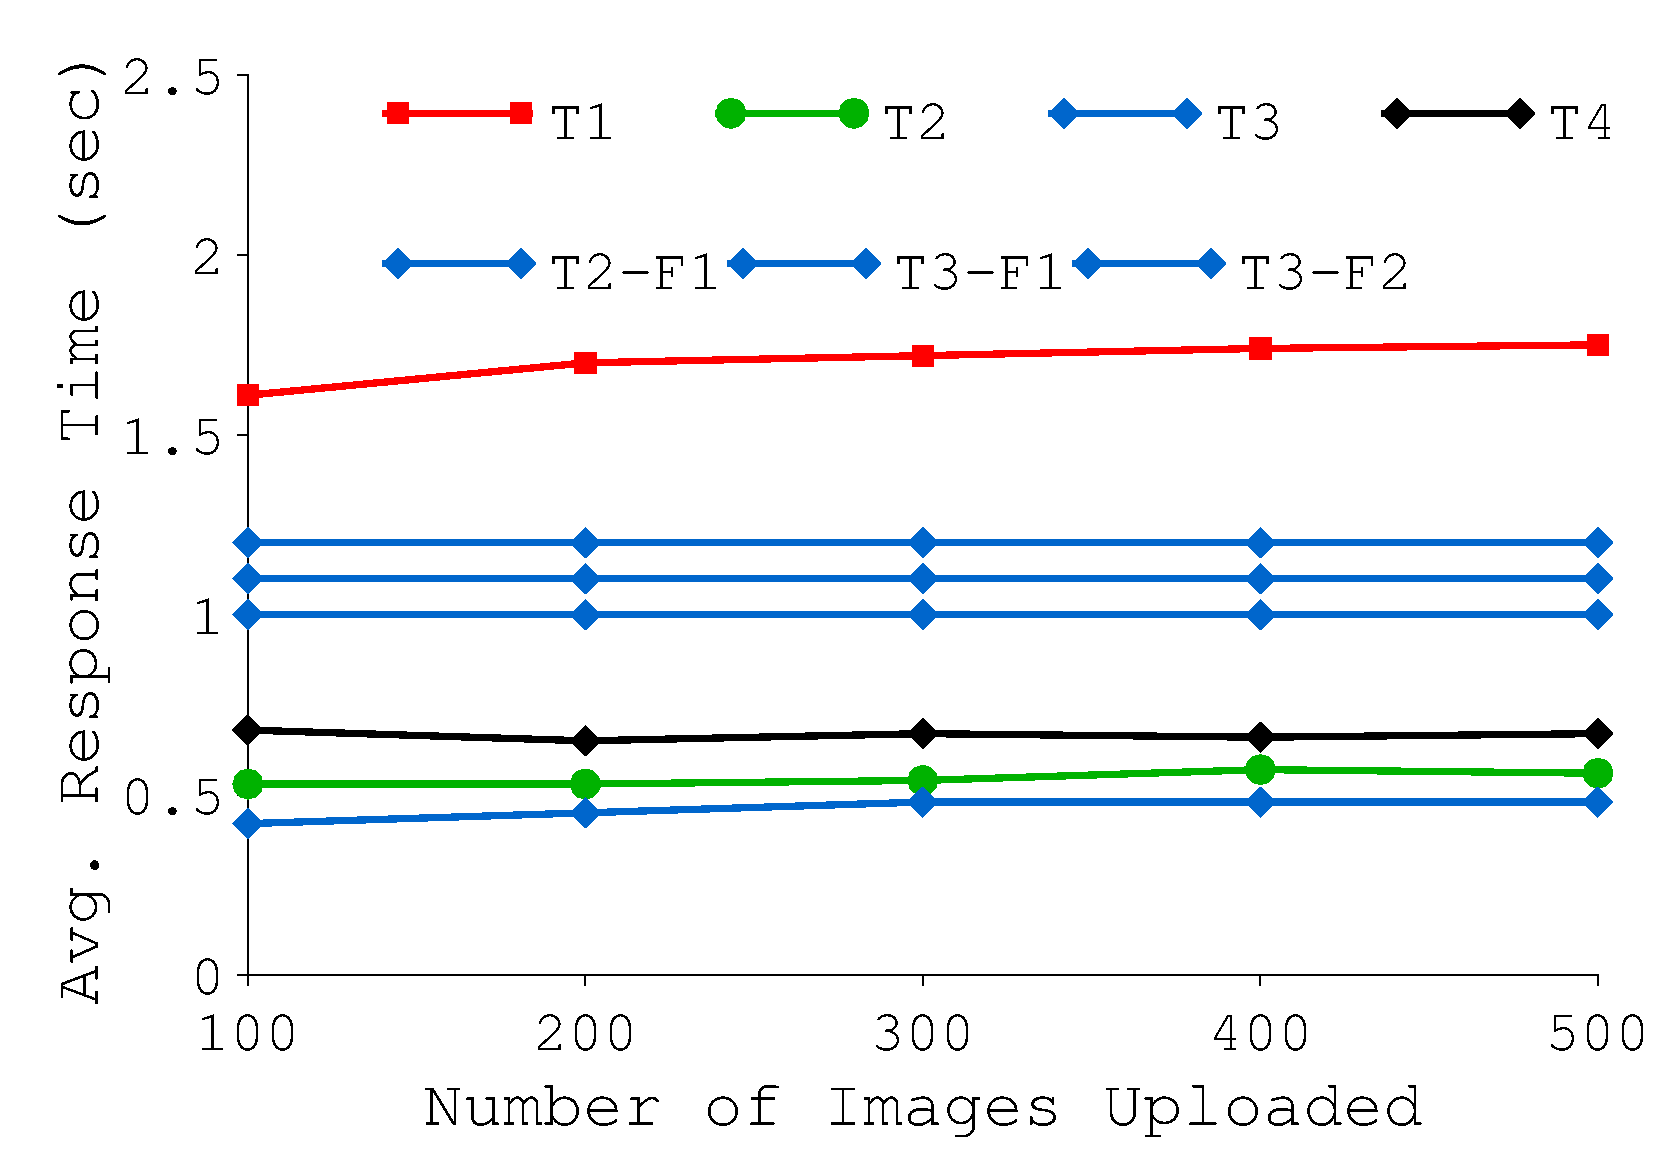
\includegraphics[width=2.5in]{Figures/g_plot_app.pdf}}
	\mycaption{fig-app}{Average Response Time Under Different Computing Models}
	{
	}
\end{center}
\end{figure}
}



\hfill\break
\noindent \textbf{Computing Models.}
Figure~\ref{fig-app} presents the average response time of a single image under different
computing models as described in section~\ref{sec:computing-models}. The average response time including: time to upload,
time for computation, possibly time for job migration, and time for return message.
Images are uploaded in a batch fashion. Computation and migration on edge device start
right after all images have been uploaded. It is clear that T3 has the best overall performance
over other computing models. This result confirms our simulation result presented in section~\ref{sec:simulation}.
T4 is better than T1 because our server has much stronger processing power than our Macbook,
which offsets the gain of edge device's fast network.
The response time of T1 and T4 stay constant even number of images increases is due to the
limitations we described above. Both T2 and T3 perform better than T4, because they have the option to
offload jobs to cloud server while having an extra parallelism on edge devices compared with T4.
In our development, T2 and T3 are using the same load-balancing algorithm described
in section~\ref{sec:load-balancing}. Due to the limitations of testbed setup, we fail to skip the
initial warmup period: migration code will calculate the best migration candidates after uploading finished,
where each edge's local copy of other \(EW\)s are all zero. Given the constant estimated run time of each job and network delay,
the percentage of jobs migrated to peer edge device or cloud stay constant too.
This explains why average response time of T2 and T3 remain constant while number of images uploaded increases.
Due to the limited time and extra engineering work needed, we are not able to present more results for after-warmup period.
We leave this for future work.

\hfill\break
\noindent \textbf{Failure Models.}
Figure~\ref{fig-app} also shows the performance comparison of T2 and T3 with failures manually injected in the middle.
The failure models follow the category of section~\ref{sec:failure-models}. T2-F1 is the case where egde device failed
during computation. T3-F1 is the case where the edge device received the uploaded images failed. T3-F2 is the case where
peer edge device failed. We emulate the edge device failure by manually killing the edge process.
Since we upload images in batch, failures must be injected after images have been uploaded while computation or migration is in progress.
Otherwise the failure of edge device will not have any effect.
Therefore, we choose to inject failure 30 seconds after images have been uploaded.
However, we don't consider cloud failure here because we envision cloud has robust failure-masking techniques.
As we described above, return messages are sent back in a per-image basis, mobile application can detect remote failures by monitoring the finished jobs.
When job failure is detected by software timeout, mobile application will resend the images again to cloud server. We choose to always resend images
back to cloud even in T3 since we did not have the mechanism to tell which edge failed.
The results in Figure~\ref{fig-app} show that even in the face of failures, T2 and T3 still have better performance than T1.
In all T2-F1, T3-F1 and T3-F2 cases, as the number of images uploaded increases,
the effect of failure increases too. This is because migration happens at the very beginning. Moreover, the time of migrating increases while number of images increases.
Thus, with a fixed failure time (i.e. 30 seconds in our testing), the number of finished jobs by the failure time descreases, which implies mobile application needs to resend more images again. This explains why the average response time increases while number of images becomes larger.

\hfill\break
\noindent \textbf{Future Work.}
Application-specifc edge device runtime requires the application developer to manage all runtime details.
Even though we have implemented the basic functionalities to achieve resilient edge computing, we still
lack several components in our system. For example, the first-run-deploy subsystem, which will help
to deploy the runtime on edge device. Also some advertising techniques for mobile devices to discover
online edge devices nearby. We are aware of the limitations in current implementation, we hope we could have
more time to extend this work.
